Направление электронного образования крайне популярно и имеет важную экономическую роль.


Платформы обучения языкам(ICT) \begin{itemize}
    \item Revita \cite{katinskaia2018revita}
\end{itemize}


\begin{figure}[h]
    \centering
    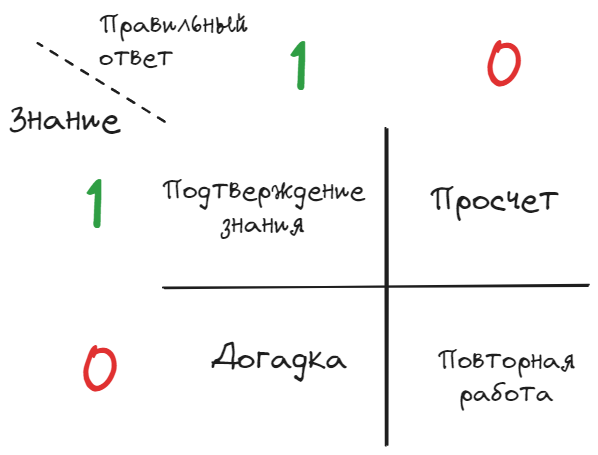
\includegraphics[width=0.5\textwidth]{assets/work/rating/bkt.excalidraw.png}
    \caption{Матрица исходов модели Байесовской оценки на шаге t}
    \label{bkt}
\end{figure}


Алгоритмические методы позволяют разрешать классические проблемы образования, включающие \begin{itemize}
    \item адаптивное составление методической литературы,
    \item \textit{прокторинг} пресечение недобросовестной кооперации обучающихся при  индивидуальном контроле знаний 
    \item формирование индивидуальной образовательной траектории.
\end{itemize}

В образование интеллектуальные ассистенты применяются \begin{itemize}
    \item  для обучения русском языку \cite{аль2019интеллектуальный}
    \item рисования поясняющих графиков \cite{bulusuautomated}
\end{itemize}



Merlin Mind - ассистент направленный целиком на образовании. Взаимодействие с ассистентом выполняется через пульт, который воспринимает речь и имеет опции по управлению презентацией.
Merlin Mind имеют открытую версию большой языковой модели, обученной на данных подготовленных с учетом общеобразовательной программы США.
